\chapter{Raport końcowy}
\label{cha:raport}

\section{Wykorzystane technologie}
\label{sec:technologie}

W naszym projekcie głównymi technologiami, które użyliśmy są: Grails (Back-end), Vaadin (Front-end) oraz Postgresql (Baza danych). Głównym kryterium podczas wyboru technologii była dla nas prostota ich nauki oraz użycia, ponieważ wcześniej mieliśmy mały kontakt z tworzeniem aplikacji webowych. Wybór bazy danych nie było kluczowy ponieważ znając język zapytań SQL praktycznie moglibyśmy operować na każdej bazie, natomiast wybór tej konkretnej był podyktowany jej znajomością przez wszystkich członków zespołu. 

Dużo więcej czasu poświęciliśmy na wybór odpowiednich frameworków do back i front endu. Po przeczytaniu paru opisów i możliwości danych narzędzi pierwszy wybór padł na framework "Grails", który nie jako wywodzi się z Ruby on Rails (w tym wypadku Groovy on Rails). Twórcy Grails zamiast budować własną warstwę komunikacji z bazą danych czy zupełnie nowy silnik szablonowego wyświetlania stron oparli się na technologiach istniejących od dłuższego czasu, sprawdzonych w systemach produkcyjnych. 

Dzięki takiej strukturze Grails nie zmusza do wdrażania nowych serwerów. Aplikacje pisane przy użyciu frameworka można wdrażać przy użyciu tradycyjnych plików *.war (na przykład na Tomcata). Dodatkowo prostota tego narzędzia objawia się w konfiguracji wszystkich plików potrzebnych do deploy'u strony. Użytkownicy innych frameworków mogą być przyzwyczajeni do topornej konfiguracji plików *.xml w początkowej fazie tworzenia projektu , natomiast Grails już przy pierwszym utworzeniu projektu dostarcza nam pełną konfigurację dzięki której naszą stronę możemy prawie od razu wrzucić na serwer. Dodatkowo wprowadzanie zmian konfiguracyjnych w późniejszej fazie jest bardzo proste dzięki ich podziałowi na konkretne, łatwo konfigurowalne pliki *.groovy. 

\begin{figure}[h!]
\centering
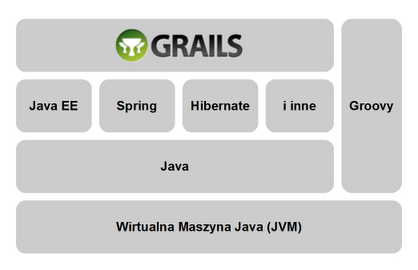
\includegraphics[width=0.5\textwidth]{./img/grails_stack}
\caption{Elementy składowe Grails}
\label{fig:grails-stack}
\end{figure}

Ponieważ grails jako warstwę widoku oferuje GSP (Groovy server pages), gdzie żeby stworzyć "coś ładnego" trzeba wykazać się sporą znajomością HTML/CSS/AJAX postanowiliśmy znaleźć prosty framework zapewniający ładny wygląd wizualny strony. Wybraliśmy framework VAADIN, który koncepcyjnie można przyrównać do Swing'a w Javie. Jest on bogaty w różnego rodzaju gotowe komponenty, których umieszczenie na stronie jest bardzo proste. Warstwa kontrolerów w przypadku użycia tego narzędzia musiała zostać zastąpiona odpowiednią obsługą event'ów, ponieważ Vaadin jest oparty na "Event-based programming". 


%%%%%%%%%%%%%%%%%%%%%%%%%%%%%%%%%%%%%%%%

\section{Implementacja bazy danych}
\label{sec:impldb}

Kolejnym atutem Grails'a jest prostota implementacji bazy danych w oparciu o ORM (Object-Relational Mapping). Podstawową składową Grails, umożliwiającą wygodną komunikację z danymi przechowywanymi w bazie jest GORM (Grails ORM). Jest on warstwą abstrakcji ponad Hibernate, czyli wykorzystuje wszystkiego jego zalety  a dodatkowo oferuje nam wiele bardzo przydatnych funkcjonalności. 

Główną zaletą GORM'a jest duża wygoda pracy oraz przejrzystość tworzonego kodu. Aby stworzyć prostą tabelę w bazie danych wystarczy utworzyć nową klasę domenową, która w wyglądzie bardzo przypomina zwykłą klasę Javy. Dodatkowo mamy do dyspozycji bardzo intuicyjne określanie ograniczeń dla konkretnych kolumn oraz kilka gotowych algorytmów tworzenia kluczy (pola ID). 

Tworzenie relacji między tabelami jest również bardzo proste ponieważ wystarczy użyć predefiniowanych zmiennych 'hasMany' oraz 'belongsTo' w odpowiednich klasach domenowych. Podczas tworzenia projektu bardzo pomocny okazał się dostęp do danych oferowany przez GORM'a, który w sposób dynamiczny tworzy funkcje dostępu do danych. Na przykład jeżeli stworzymy sobie klasę (tabelę) 'Book' z polem 'Author' to automatycznie zostaje wygenerowany szereg funkcji dostępu do danych w bazie danych typu : Dom.findAllByDateCreatedAndAuthor(date, author). Więc tak naprawdę znajomość SQL'a była w tym projekcie praktycznie nie wymagana.

Ostatnim wykorzystywanym przez nas udogodnieniem GORM'a było automatyczne datowanie. Wystarczyło w klasie domenowej stworzyć pola o nazwach 'dateCreated' lub 'lastModyfied' a GORM sam troszczył się o adekwatne uzupełnianie tych pól.

%%%%%%%%%%%%%%%%%%%%%%%%%%%%%%%%%%%%%%%%

\section{Wybrane interfejsy użytkownika}
\label{sec:interfejsy}

% TODO screeny z jakimiś opisami, ogólny wygląd strony?
\subsection{Logowanie}
\label{sec:login}
Na rysunku \ref{fig:login} przedstawione zostało okno logowania. Użytkownik podaje swój login i hasło oraz wybiera, czy chce, aby dane były zapamiętane w plikach cookies, co umożliwi pozostanie zalogowanym po ponownym włączeniu strony lub jej odświeżeniu. W przypadku gdy użytkownik zapomniał hasła, może kliknąć łącze \emph{Forgotten password? Click here} i ponownie wpisać adres e-mail, na który zarejestrowane jest konto. Dzięki temu system zresetuje hasło na losowy ciąg znaków i wyśle je do użytkownika.

\begin{figure}[h!]
\centering
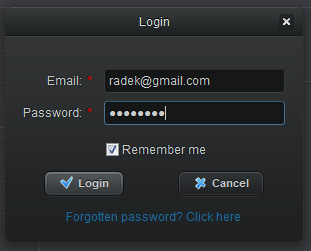
\includegraphics[width=0.5\textwidth]{./img/interfejsy/login2}
\caption{Okno logowania}
\label{fig:login}
\end{figure}

\subsection{Strona startowa}
\label{sec:start_page}

Po zalogowaniu na stronie startowej pojawiają się informacje o nadchodzących sesjach. Na rysunku \ref{fig:start_page_joined} ciemniejszym kolorem oznaczone są sesje, do których użytkownik w pełni dołączył, jaśniejszym --- oczekujące na akceptację przez założyciela ogłoszenia. Dla zalogowanych użytkowników możliwa jest nawigacja do kolejnych podstron --- zakładek.
\begin{figure}[h!]	
\centering
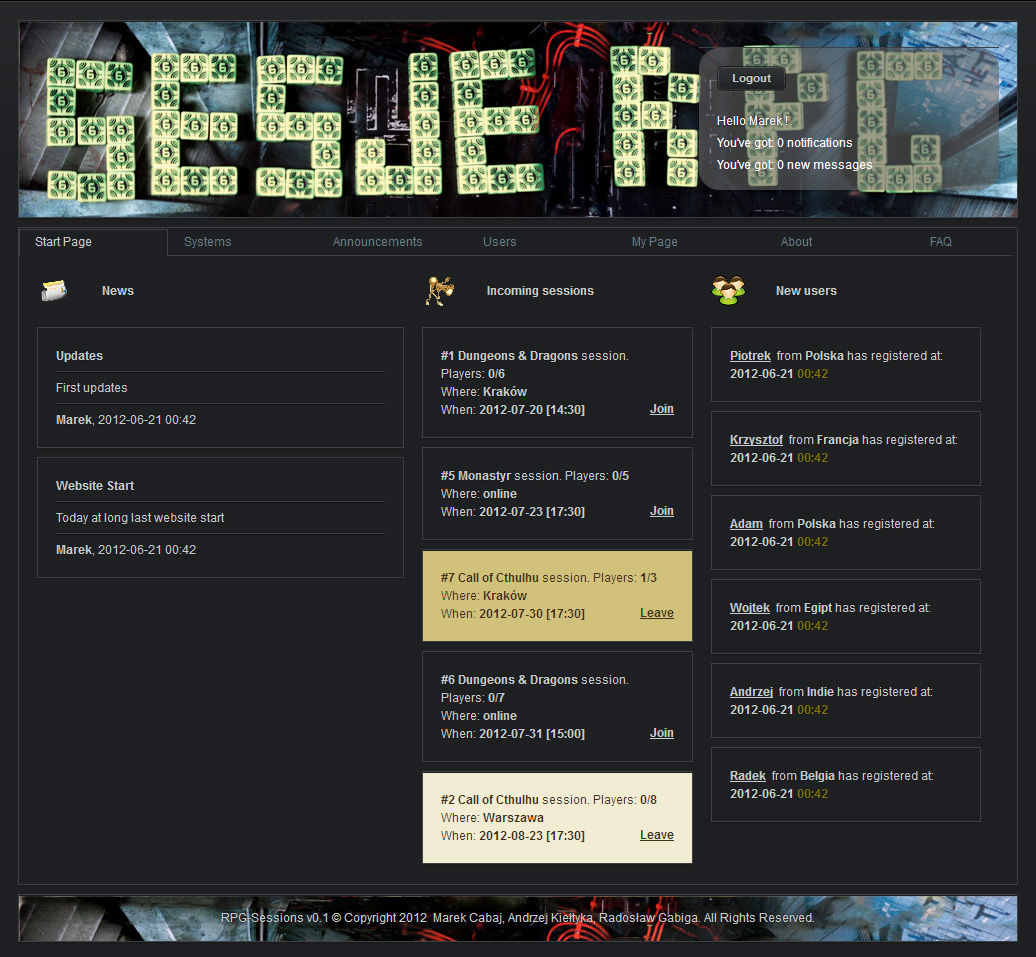
\includegraphics[width=0.9\textwidth]{./img/interfejsy/start_page_joined}
\caption{Strona startowa zalogowanego użytkownika}
\label{fig:start_page_joined}
\end{figure}

\subsection{Lista systemów}
\label{sec:systems}
Wybranie zakładki \emph{Systems} powoduje przejście do listy systemów RPG zapisanych w bazie serwisu. Składa się ona z tabeli systemów z podziałem na gatunki i rok wydania oraz opisu wybranej pozycji znajdującego się poniżej. Listę można filtrować względem pierwszej litery nazwy lub wyświetlać wszystko. Jeśli zalogowany użytkownik jest administratorem lub moderatorem, widoczne stają się przyciski \emph{New system}, \emph{Edit} i \emph{Delete} służące kolejno do dodawania nowego systemu, edycji istniejącego oraz usuwania. Całość przedstawia rysunek \ref{fig:systems}.

\begin{figure}[h!]
\centering
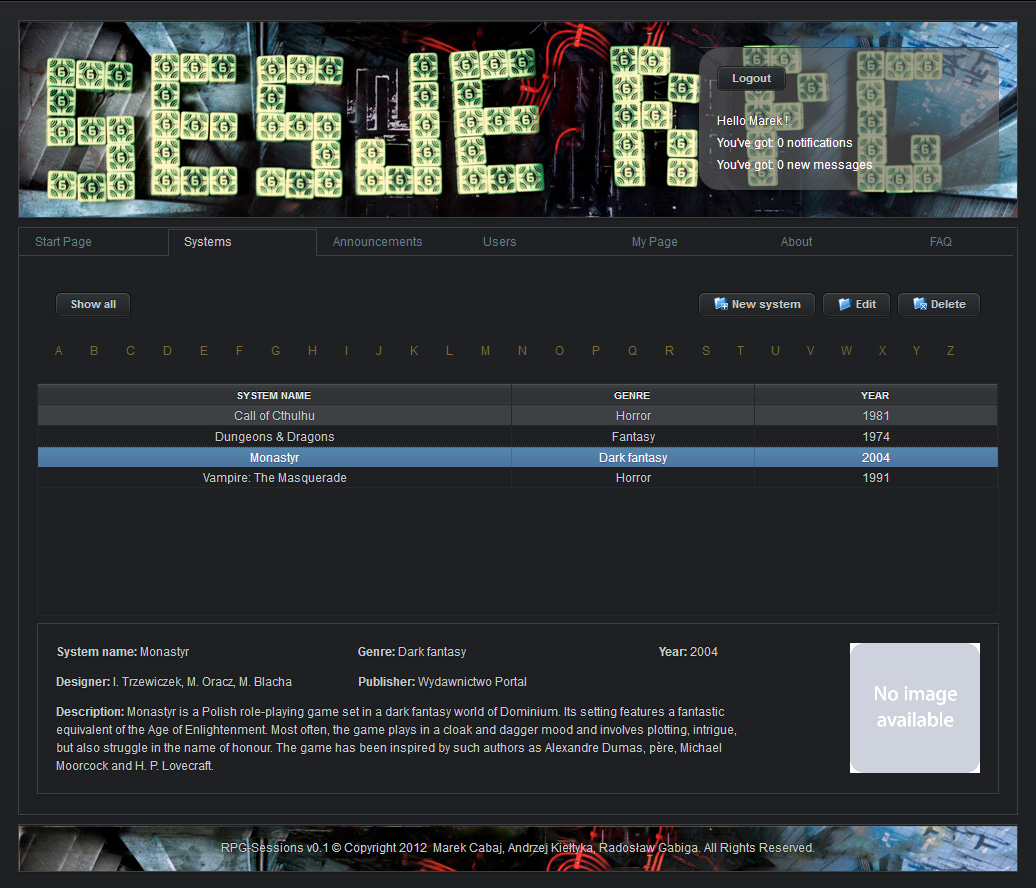
\includegraphics[width=0.9\textwidth]{./img/interfejsy/systems}
\caption{Lista systemów RPG}
\label{fig:systems}
\end{figure}

\subsection{Ogłoszenia}
\label{sec:sessions}
Zakładka \emph{Announcements} stanowi główny cel serwisu --- ogłoszenia o odbywających się sesjach (rys. \ref{fig:sessions}).  Znajduje się tutaj tabela z kluczowymi informacjami oraz rozwinięcie dostępne po zaznaczeniu wybranej pozycji. Sesje oznaczane są takimi samymi kolorami jak na stronie startowej. Po wybraniu sesji i naciśnięciu przycisku \emph{Join} pojawia się okno wyboru pozycji w~trakcie sesji (rys. \ref{fig:join_session}). Można dołączyć jako Mistrz Gry (\emph{Master}) lub jako Gracz (\emph{Player}). W~przypadku gdy dołączający użytkownik nie jest założycielem ogłoszenia, po wyborze pozycji wysyłana jest wiadomość z prośbą o akceptację do osoby odpowiedzialnej za sesję. 

\begin{figure}[h!]
\centering
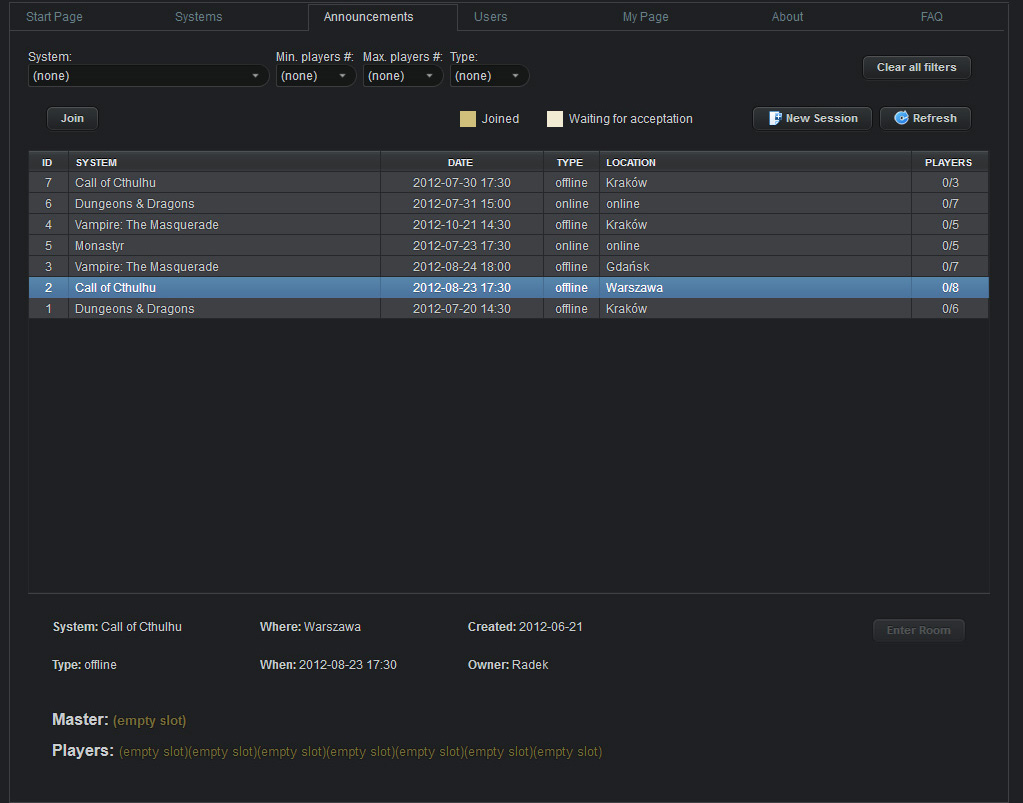
\includegraphics[width=0.9\textwidth]{./img/interfejsy/sessions}
\caption{Lista ogłoszeń}
\label{fig:sessions}
\end{figure}

Po naciśnięciu przycisku \emph{New Session} pojawia się okno tworzenia nowej sesji. Użytkownik podaje wymagane dane, wybiera czy od razu chce do niej dołączyć jako Gracz lub Mistrz Gry i dodaje ogłoszenie do bazy. Formularz ten jest przedstawiony na rysunku \ref{fig:create_session}.

\begin{figure}[h!]
\centering
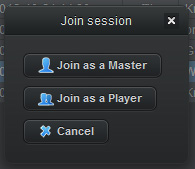
\includegraphics[width=0.3\textwidth]{./img/interfejsy/join_session}
\caption{Dołączanie do sesji}
\label{fig:join_session}
\end{figure}

\begin{figure}[h!]	
\centering
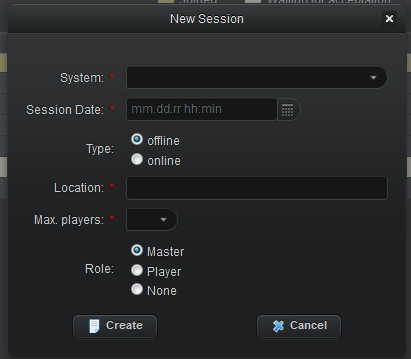
\includegraphics[width=0.7\textwidth]{./img/interfejsy/create_session}
\caption{Tworzenie nowej sesji}
\label{fig:create_session}
\end{figure}


%waiting for accepation ???


\subsection{Lista użytkowników}
\label{sec:users_detail}
Zakładka \emph{Users} (rys. \ref{fig:users_details} to lista użytkowników zamierająca pseudonim, datę dołączenia, kraj pochodzenia oraz status konta (aktywne, nieaktywne). Użytkownicy mogą wyświetlić szczegóły profilu po wybraniu danej osoby i naciśnięciu \emph{Show details}. Gdy zalogowany jest administrator lub moderator, widoczny jest również przycisk \emph{Deactivate account} służący do banowania użytkowników. 

\begin{figure}[h!]	
\centering
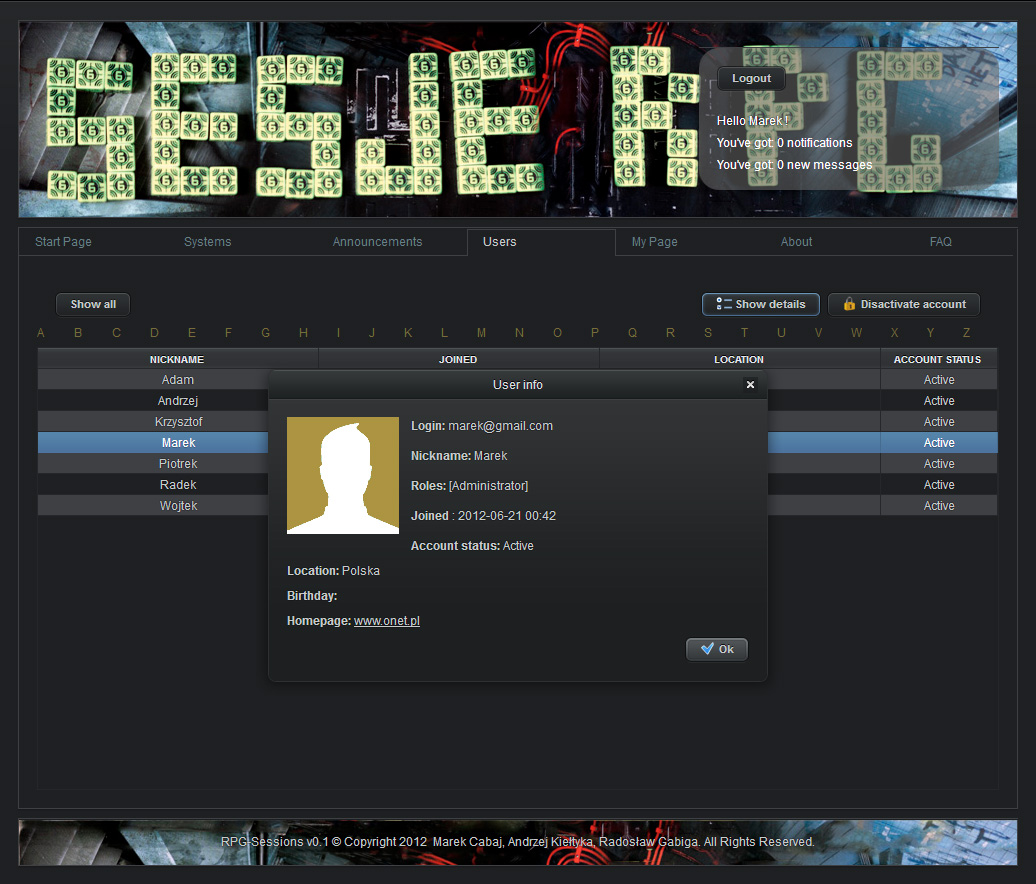
\includegraphics[width=0.9\textwidth]{./img/interfejsy/users_details}
\caption{Szczegóły profilu użytkownika}
\label{fig:users_details}
\end{figure}

\subsection{Strona profilowa}
\label{sec:my_page}
Zakładka \emph{My Page} zawiera profil zalogowanego użytkownika. Może tutaj przeglądać i edytować dane profilowe, sprawdzać wiadomości i powiadomienia systemowe, przeglądać sesje, w których uczestniczy, oczekuje na akceptacje lub które stworzył. Ponadto można tworzyć scenariusze rozgrywek jak i (w przyszłości) karty postaci. Administrator dodatkowo posiada możliwość dodawania wiadomości na stronę główną (\emph{News}) i pytań w dziale \emph{FAQ}. Przykład profilu ze stworzonymi sesjami przedstawia rysunek \ref{fig:mypage_sessions}.

\begin{figure}[h!]	
\centering
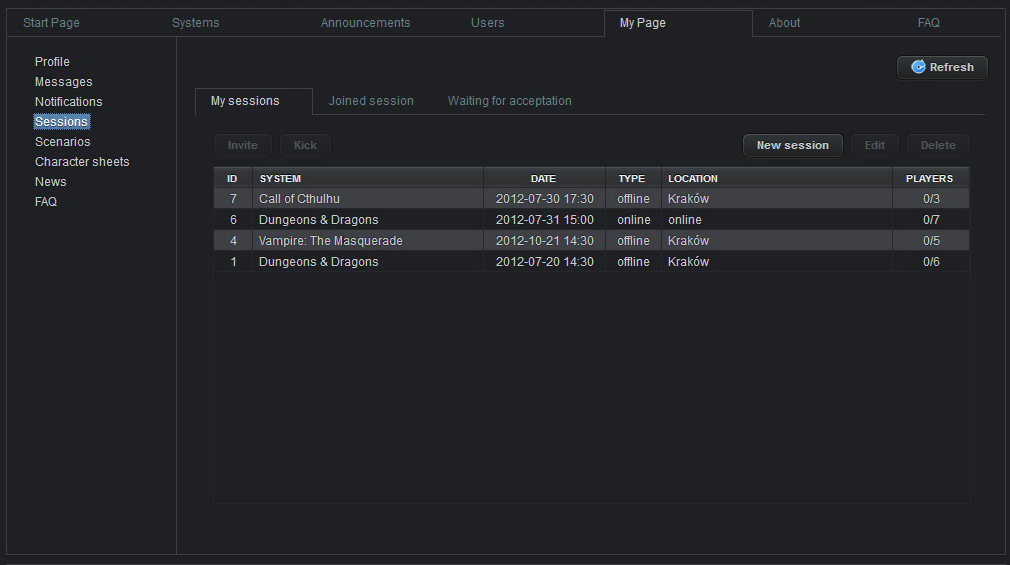
\includegraphics[width=0.9\textwidth]{./img/interfejsy/mypage_sessions}
\caption{Sesje użytkownika}
\label{fig:mypage_sessions}
\end{figure}

\subsection{FAQ}
\label{sec:faq}

\begin{figure}[h!]	
\centering
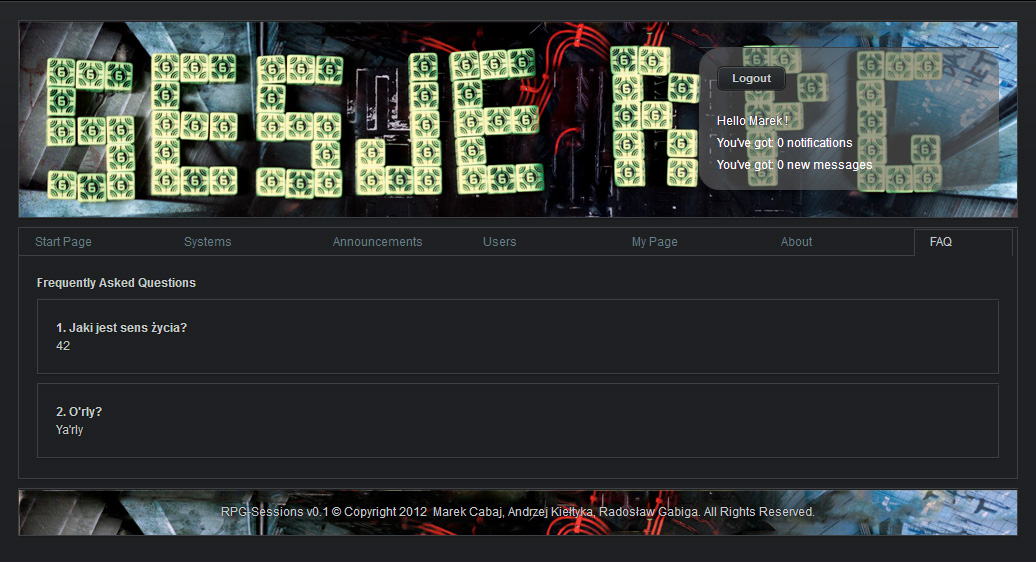
\includegraphics[width=0.9\textwidth]{./img/interfejsy/faq}
\caption{FAQ}
\label{fig:faq}

\end{figure}
Ostatnią zakładką, przedstawioną na rysunku \ref{fig:faq} są najczęściej zadawane pytania - \emph{FAQ}. Administrator systemu dodaje pozycje ze swojej strony profilowej.

\subsection{Edytowanie}
\label{sec:edit}
Osoba z odpowiednimi uprawnieniami może edytować niektóre elementy serwisu --- systemy RPG, wiadomości, FAQ itp. Każdy z tych formularzy wygląda podobnie, edytować można wszystkie dane uzupełniane przy tworzeniu. Przykład edycji systemu RPG znajduje się na rysunku \ref{fig:edit}.

\begin{figure}[h!]	
\centering
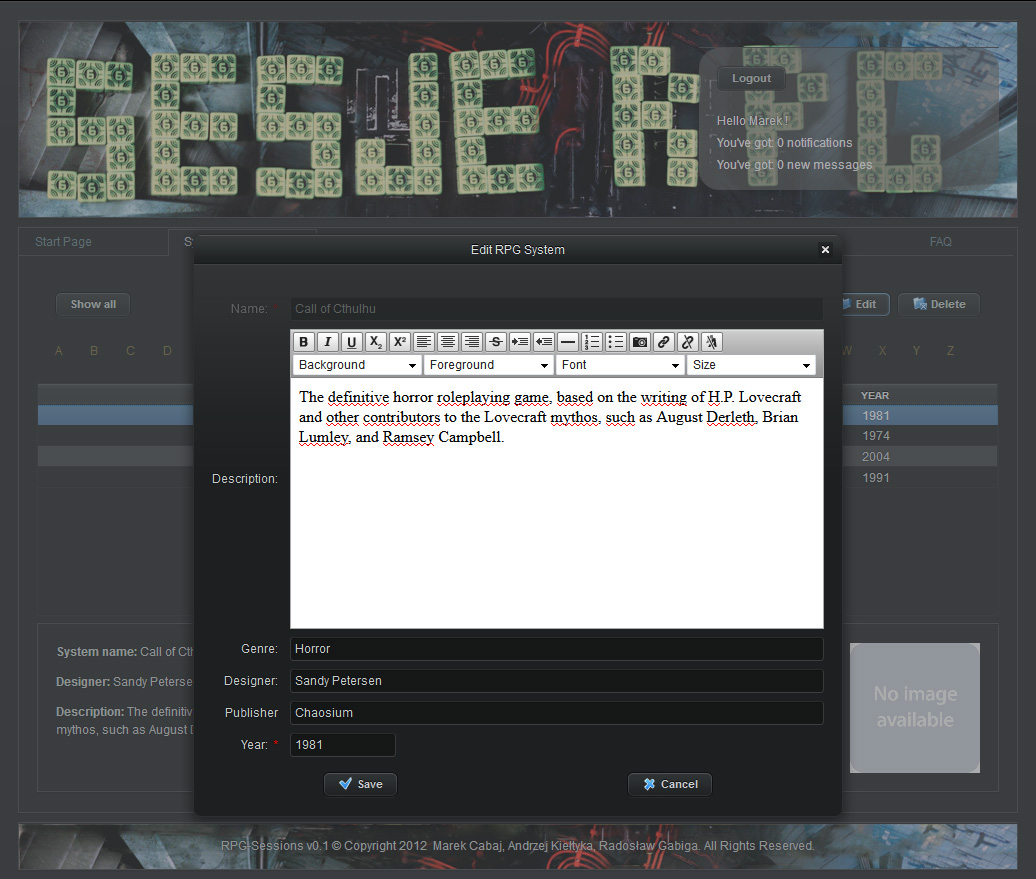
\includegraphics[width=0.9\textwidth]{./img/interfejsy/edit}
\caption{FAQ}
\label{fig:edit}
\end{figure}

\subsection{Chat}
\label{sec:chat}

W przypadku sesji online aktywny staje się przycisk \emph{Enter Room}. Umożliwia on wejście do pokoju z chatem z innymi uczestnikami sesji. Poza typową funkcjonalnością rozmawiania istnieje przycisk \emph{Shot history} wyświetlający wiadomości napisane przed dołączeniem danego użytkownika do kanału (przed otwarciem okna rozmowy) oraz przycisk \emph{Throw a dice} symulujący rzut kością k12, czyli losujący liczbę z zakresu 1--12. W przyszłości dodane będą rzuty parametryzowane --- wybór ilości kości (rzutów) i ich ilość ścian.

\begin{figure}[h!]	
\centering
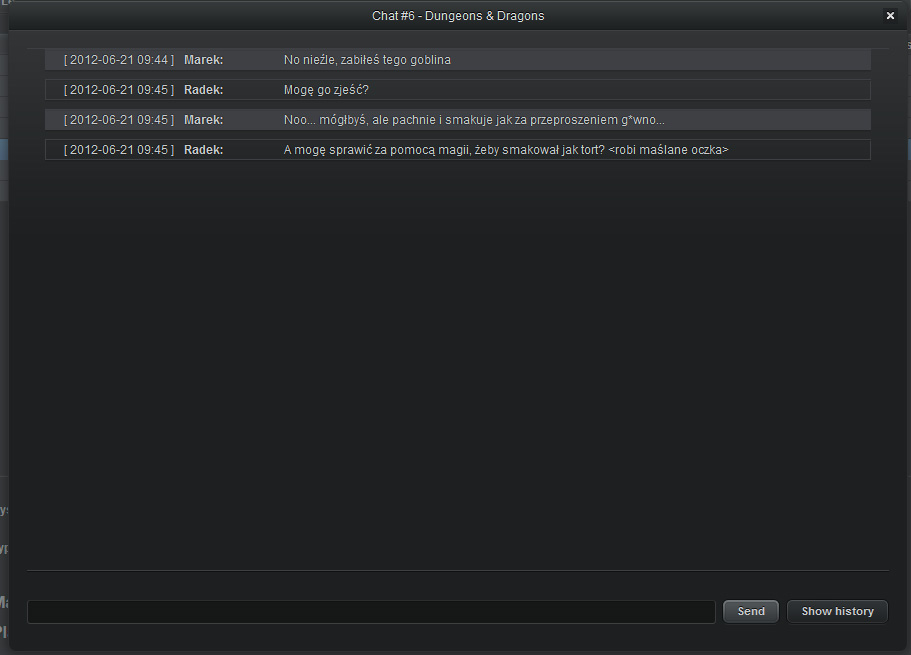
\includegraphics[width=0.9\textwidth]{./img/interfejsy/chat}
\caption{Chat}
\label{fig:faq}
\end{figure}

%%%%%%%%%%%%%%%%%%%%%%%%%%%%%%%%%%%%%%%%

\section{Różnice pomiędzy projektem oraz implementacją}
\label{sec:roznice}

% TODO wszelkie różnice, zmiany

%%%%%%%%%%%%%%%%%%%%%%%%%%%%%%%%%%%%%%%%

\section{Rozwijanie i modyfikowanie aplikacji}
\label{sec:rozwoj}

Aplikację webową opracowaną w ramach niniejszego projektu można rozwijać w wielu kierunkach. Poniżej znajduje się lista wybranych możliwości modyfikacji:
\begin{itemize}
\item implementacja niezrealizowanych funkcjonalności serwisu, m.in. modułu tworzenia kart postaci
\item internacjonalizacja serwisu,
\item opracowanie profesjonalnego layoutu głównego dla aplikacji,
\item dodanie do witryny stylów tematycznych związanych z poszczególnymi systemami RPG,
\item rozdzielenie profilu na stronie użytkownika na: podgląd profilu, dane profilu oraz ustawienia konta/prywatności,
\item dodanie możliwości nadawania uprawnień moderatora użytkownikom przez administrację serwisu,
\item dodanie większej ilości funkcji społecznościowych, np. listy znajomych,
\item optymalizacja kodu witryny.
\end{itemize}

%%%%%%%%%%%%%%%%%%%%%%%%%%%%%%%%%%%%%%%%

\section{Wnioski}
\label{sec:doswiadczenia}

% TODO wnioski
